\documentclass[12pt]{article}

% PAQUETES IMPORTADOS
\usepackage[utf8]{inputenc}                     %input encoding
\usepackage[a4paper, margin=2.5cm]{geometry}    %margins
\usepackage{sectsty}                            %tamanos de cabeceras
\usepackage[spanish,es-tabla]{babel}            %espanol
\usepackage{fontspec}                           %fuentes
\usepackage{anyfontsize}                        %tamanos de fuentes
\usepackage[style=ieee]{biblatex}               %bibliografia
\usepackage{csquotes}                           %citas a bibliografia
\usepackage{nameref}                            %referencia a capitulos
\usepackage{amsmath}                            %inline maths
\usepackage{amssymb}                            %math symbols
\usepackage{graphicx}                           %imagenes
\usepackage{color}                              %colores de fuentes
\usepackage{hyperref}                           %enlaces
\usepackage{ulem}                               %subrayados decentes
\usepackage{titlesec}                           %tamaños de títulos

% PROPIEDADES DE PAQUETES
\hypersetup{    % Color de enlaces (usados para referencias a capítulos)
    colorlinks,
    citecolor=black,
    filecolor=black,
    linkcolor=black,
    urlcolor=black
}

%tamaños de títulos
\titleformat*{\section}{\Huge\bfseries}
\titleformat*{\subsection}{\LARGE\bfseries}
\titleformat*{\subsubsection}{\large\bfseries}

% ARCHIVOS Y CARPETAS AUXILIARES
\graphicspath{ {./images/} }
\addbibresource{biblio.bib}

% FUENTES
\renewcommand{\contentsname}{Índice de Contenidos}
\setmainfont{Times New Roman}
\sectionfont{\fontsize{20pt}{15}\selectfont}
\subsectionfont{\fontsize{18pt}{15}\selectfont}
\subsubsectionfont{\fontsize{16pt}{15}\selectfont}

\begin{document}

%---------------------------------------------------
% PORTADA
%---------------------------------------------------
\begin{titlepage}
\begin{flushright}
\hfill\parbox[r][][c]{0.5\textwidth}{
{\fontsize{14}{14}\selectfont Universidad de Valladolid \\
E.T.S Ingeniería Informática \\
Grado en Ingeniería Informática\\
Rama de Ingeniería de Software\\
Cuarto Curso}}

\end{flushright}

\vfill
\centering
{\fontsize{16pt}{1cm}\selectfont \textbf{Resumen de los Apuntes de la Asignatura <<Planificación y Gestión de Proyectos>>}}


\vfill
\begin{flushright}
\hfill\parbox[r][][c]{0.4\textwidth}{
{\fontsize{14pt}{14cm}\selectfont
Bayón Sanz, Miguel
}
}
\end{flushright}

\end{titlepage}

%---------------------------------------------------
% INDICE
%---------------------------------------------------
\tableofcontents
\newpage

%---------------------------------------------------
% CUERPO
%---------------------------------------------------

%---------------------------------------------------
% Seccion 1
%---------------------------------------------------
\newpage
\section{Introducción a la gestión de proyectos Software}
\label{1.0.0}
\subsection{Introducción}
\label{1.1.0}

{Los proyectos de Software, al igual que otros proyectos, se basan en cumplir una serie de objetivos para satisfacer necesidades reales. Esto se hará encontrando a los inversores y sus objetivos. La gestión de proyectos tiene como finalidad cumplir sus objetivos, conociendo el estado del mismo proyecto en todo momento.}

\subsection[¿Por qué es importante la gestión de proyectos de Software?]{¿Por qué es importante la gestión de proyectos de Software?}
\label{1.2.0}

{Los proyectos de Software son el tipo de proyecto que más dinero mueve, implicando que una mala gestión haga que se pueda perder todo ese dinero. Según un estudio, de entre 13.522 proyectos:}

\begin{itemize}
    \item {El 66\% fracasa.}
    \item {El 82\% terminan tarde.}
    \item {El 43\% excede el presupuesto.}
\end{itemize}

\subsection{¿Qué es un proyecto?}
\label{1.3.0}

{Un proyecto es una \textbf{actividad planeada} que cuenta con la definición de todos los pasos y de su duración. Este cuenta también con una definición oficial establecida en el BSO ISO 10006 (1997): \textit{Proceso único consistente en un conjunto de actividades coordinadas y controladas con fechas de inicio y fin, promovido para conseguir un objetivo conforme a requisitos específicos incluyendo restricciones de tiempo, coste y recursos}.} \bigskip

{El proyecto se encuentra en un término medio entre un trabajo rutinario y una investigación. Para diferenciarlos, debe cumplir los siguientes puntos:}

\begin{itemize}
    \item {Debe contener \textbf{tareas no rutinarias}.}
    \item {Requiere \textbf{planificación}.}
    \item {Debe cumplir \textbf{objetivos específicos}.}
    \item {Se debe completar en un \textbf{periodo de tiempo}.}
    \item {El trabajo se realiza \textbf{para otra persona}.}
    \item {Implica \textbf{varias especialidades}.}
    \item {Los empleados formarán un \textbf{grupo de trabajo temporal}.}
    \item {El trabajo se llevará a cabo en \textbf{varias fases}.}
    \item {Los \textbf{recursos} del proyecto estarán \textbf{limitados}.}
    \item {Debe ser un proyecto \textbf{grande y/o complejo}.}
\end{itemize}

{El tamaño del equipo es especialmente importante, porque implicará una mayor organización entre los participantes. Además, toda la experiencia ganada como equipo \textbf{se perderá al disolverse} el mismo (al ser grupos temporales).}

\subsection[Proyectos de Software vs otros tipos de proyectos]{Proyectos de Software vs otros tipos de \\proyectos}
\label{1.4.0}

{Algunas características de los proyectos de Software los hacen especialmente complicados:}

\begin{itemize}
    \item {\textbf{Invisibilidad}: el progreso no es inmediatamente visible.}
    \item {\textbf{Complejidad}: el proyecto de Software tiene gran complejidad por unidad monetaria.}
    \item {\textbf{Conformidad}: los desarrolladores se tienen que conformar con los requisitos de los clientes, que pueden ser cambiantes e inconsistentes.}
    \item {\textbf{Flexibilidad}: los sistemas Software están sujetos al cambio para acomodarse a elementos externos.}
\end{itemize}

\subsection[Gestión de contratos y gestión de proyectos técnicos]{Gestión de contratos y gestión de proyectos \\técnicos}
\label{1.5.0}

{En los proyectos internos se desarrolla para la misma organización. En los externos, al haber un contrato entre cliente y proveedor, existirán dos gestores de proyectos: uno del lado del cliente y otro del lado del proveedor. El del cliente (gestor del contrato) se ocupará de comprobar que el proyecto cumpla con los plazos y se ajuste al presupuesto, mientras que el del proveedor se ocupará de las decisiones de carácter técnico del proyecto.}

\subsection[Actividades cubiertas por la gestión de proyectos de Software]{Actividades cubiertas por la gestión de \\proyectos de Software}
\label{1.6.0}

{Un proyecto de Software suele pasar por \textbf{tres procesos} para generar un nuevo sistema:}

\begin{itemize}
    \item {\textbf{Estudio de viabilidad}: se evalúa lo que se quiere conseguir con sus requisitos y se comprueba que el proyecto sea viable. Si el proyecto es grande, el estudio de viabilidad puede ser un proyecto en sí mismo.}
    \item {\textbf{Planificación}: si el proceso anterior tiene un resultado positivo puede comenzar la planificación. Para proyectos muy grandes, la planificación no se detalla desde el principio, sino que se genera un guion general para todo el proyecto y se detalla solamente la primera etapa, dejando el resto para cuando se llegue a ellas.}
    \item {\textbf{Ejecución de proyecto}: El proyecto se ejecuta, a veces con sub-secciones de diseño e implementación. El libro, además, recalca la diferencia entre planificación (detallado de las actividades a llevar a cabo para generar un producto) y el diseño (decisiones sobre la forma del producto final).}
\end{itemize}

{Durante el proceso de implementación, surgirán actividades como las siguientes:}

\begin{itemize}
    \item {\textbf{Análisis de requisitos}: funciones o calidad mínima que serán requeridas por los usuarios del sistema.}
    \item {\textbf{Diseño de arquitectura}: Selección de los componentes (Software, Hardware o proceso de trabajo) que cumplirán cada requisito.}
    \item {\textbf{Diseño detallado}: Se diseñan independientemente las unidades que compondrán cada componente Software.}
    \item {\textbf{Programar y testear}: Escritura y depuración de cada unidad.}
    \item {\textbf{Integración}: Se prueban los componentes juntos.}
    \item {\textbf{Prueba de cualificación}: Se comprueba que todos los requisitos se cumplen.}
    \item {\textbf{Instalación}: El sistema trabaja en condiciones reales y/o para clientes.}
    \item {\textbf{Soporte de aceptación}: Resolución de errores en el sistema funcional. Una resolución de error puede ser un proyecto completo.}
\end{itemize}

\subsection{Planes, métodos y metodologías}
\label{1.7.0}

\begin{itemize}
    \item {\textbf{Metodología}: Conjunto de métodos.}
    \item {\textbf{Método}: Forma de trabajar o de organizar el trabajo.}
    \item {\textbf{Plan}: Organización de las tareas de un proyecto siguiendo una serie de métodos.}
\end{itemize}

\subsection{Algunas maneras de clasificar los proyectos de Software}
\label{1.8.0}

{Algunos factores a tener en cuenta al diseñar un proyecto son:}

\begin{itemize}
    \item {\textbf{Usuarios obligados contra usuarios voluntarios}: Un producto de uso empresarial contra un videojuego.}
    \item {\textbf{Sistemas de información contra sistemas embebidos}: Control de información contra control de máquinas.}
    \item {\textbf{Objetivos contra productos}: Solucionar un problema contra crear un nuevo sistema.}
\end{itemize}

\subsection{Stakeholders}
\label{1.9.0}

{Son aquellos que tienen un interés o una implicación directa en el proyecto o que se beneficiarán de él. Pueden ser:}

\begin{itemize}
    \item {Miembros del equipo del proyecto}
    \item {Externos al equipo del proyecto pero pertenecientes a la misma organización}
    \item {Externos a la empresa}
\end{itemize}

{Un buen líder de proyecto tiene que tratar de buscar los intereses de estos stakeholders y plasmarlos en el proyecto, buscando que todos obtengan beneficio de ello (La <<Theory W>> de Boehm and Ross, la situación \textit{win-win}).}

\subsection{Estableciendo objetivos}
\label{1.10.0}

{Algunos stakeholders serán los financiadores del proyecto y que además serán dueños del resultado y establecerán objetivos.} \bigskip

{Los objetivos se definen como post-condiciones del proyecto que deben ser cumplidas para que el proyecto pueda tener éxito (por ejemplo, <<nuestro proyecto tendrá éxito si el cliente puede comprar productos online>>.} \bigskip

{En caso de que varios stakeholders puedan tener derecho a la propiedad del proyecto, se establece una autoridad (generalmente un \textit{comité de dirección de proyecto}) con la potestad de establecer, vigilar y modificar objetivos. El líder de proyecto tendrá que reportarle los avances.}

\subsubsection{Sub-objetivos o metas}
\label{1.10.1}

{Al ser algunos objetivos muy generales (<<\textit{el proyecto será un éxito si reduce el consumo de energía}>>), se suelen dividir en sub-objetivos o metas fáciles de interpretar (<<\textit{para alcanzar este objetivo, será necesario...}>>).} \bigskip

{Se suele definir un objetivo bien definido con el acrónimo \textbf{SMART}:}
\begin{itemize}
    \item {\textbf{S}pecific o específico: es concreto y está bien definido.}
    \item {\textbf{M}easurable o medible: debe ofrecer medidas (como \textit{reducir} o \textit{reducir en X unidad}) en lugar de conceptos abstractos (como \textit{mejorar}).}
    \item {\textbf{A}chievable o lograble.}
    \item {\textbf{R}elevant o relevante en cuanto al propósito del proyecto.}
    \item {\textbf{T}ime constrained o restringido en el tiempo: se tiene que poder completar en un tiempo determinado.}
\end{itemize}

\subsubsection{Medidas de efectividad}
\label{1.10.2}

{Las medidas de efectividad ofrecen una forma práctica de comprobar el cumplimiento de un objetivo.}

\subsection{Business case o Caso de negocio}
\label{1.11.0}

{El Business case forma parte del estudio de viabilidad y consiste en un análisis contrastado de coste-beneficio y cuándo se conseguirá ese beneficio.} \bigskip

{Los planes de proyecto deben asegurarse de que el Business case se mantiene intacto.}

\subsection{Éxito y fracaso de un proyecto}
\label{1.12.0}

{Un proyecto de Software suele ser un éxito si cumple:}

\begin{itemize}
    \item {Con la funcionalidad acordada.}
    \item {Con el nivel de calidad requerido.}
    \item {Que acaba a tiempo.}
    \item {Que acaba dentro del presupuesto acordado.}
\end{itemize}

{A veces, puede cumplir con estos términos pero no cumplir con el Business case (los beneficios superan los gastos). Esto significaría que el proyecto es un éxito pero es un fracaso empresarial, al igual que puede ocurrir que un proyecto sea un fracaso por romper varios puntos anteriores pero supere con creces el Business Case.} \bigskip

{El Business Case busca presentar cuáles son los objetivos de negocio. Estos objetivos se pueden acercar a los objetivos de proyecto mediante actividades como evaluaciones de mercado o de usuarios.} \bigskip

{Los proyectos, aun fracasando, pueden implicar adquisición de conocimientos o una mejor relación con el cliente que pueden llevar a que futuros proyectos puedan ser un éxito o puedan generar mejores ingresos.}

\subsection{¿Qué es la gestión?}
\label{1.13.0}

{Gestionar en un proyecto es:}

\begin{itemize}
    \item {Planificar tareas.}
    \item {Conseguir a los empleados adecuados.}
    \item {Dirigir.}
    \item {Controlar los progresos.}
    \item {Tomar medidas para remediar parones.}
    \item {Intervenir con los stakeholders.}
\end{itemize}

\subsection{Control de gestión}
\label{1.14.0}

{Cuando se prueban soluciones para resolver atascos en el proyecto, se debe monitorizar si estas soluciones dan o no resultado y buscar, en caso negativo, cuál es el verdadero problema del atasco. También se debe comprobar si la solución ha generado problemas paralelos al cambiar el plan inicial de proyecto.}

%---------------------------------------------------
% Seccion 2
%---------------------------------------------------
\newpage

\section[Evaluación de proyectos y gestión de programas]{Evaluación de proyectos y gestión de \\programas}
\label{2.0.0}
\subsection{Introducción}
\label{2.1.0}

{Además de las ganancias económicas directas, hay otras formas de decidir que un proyecto merece la pena. A veces, los beneficios de un proyecto producen ganancias indirectas y pueden combinar bien con el desarrollo de otros proyectos.} \bigskip

{Este tema introducirá:}
\begin{itemize}
    \item {El desglose del \textbf{Business Case}.}
    \item {El \textbf{Programa de Proyectos}: conjunto de proyectos interrelacionados para la consecución de beneficios que no se obtendrían si se realizasen individualmente.}
    \item {El \textbf{Portfolio de Proyectos}: conjunto de programas y proyectos no necesariamente relacionados que se priorizan, seleccionan e implementan para lograr los objetivos estratégicos de la organización.}
\end{itemize}

\subsection{Un Business case}
\label{2.2.0}

{Un estudio de viabilidad, justificación de proyecto o Business case tiene como objetivo demostrar que los beneficios superarán los gastos. Suelen estar formados por los siguientes puntos:}

\begin{enumerate}
    \item {Introducción y antecedentes de la propuesta}
    \item {Proyecto propuesto}
    \item {Mercado}
    \item {Infraestructura organizacional y operacional}
    \item {Beneficios}
    \item {Esquema del plan de ejecución}
    \item {Costes}
    \item {Argumentos financieros}
    \item {Riesgos}
    \item {Plan de gestión}
\end{enumerate}

\subsubsection{Introducción y antecedentes de la propuesta}
\label{2.2.1}

{Describe un problema a ser resuelto o una oportunidad a ser explotada.}

\subsubsection{Proyecto propuesto}
\label{2.2.2}

{Breve esquema del proyecto.}

\subsubsection{Mercado}
\label{2.2.3}

{Necesario con nuevos productos. Describe la sección del mercado interesada y los posibles competidores.}

\subsubsection{Infraestructura organizacional y operacional}
\label{2.2.4}

{Describe cómo el proyecto cambiaría la estructura de la organización. Importante si implica modificar un sistema de información de una empresa.}

\subsubsection{Beneficios}
\label{2.2.5}

{Indica las ganancias o ahorros potenciales que generaría el resultado. Si el proyecto no pretende generar ganancias, convendría cuantificar el resultado.}

\subsubsection{Esquema del plan de ejecución}
\label{2.2.6}

{Contendrá un plan general del proyecto, además de otras decisiones como partes que se externalizarán a otras empresas, promoción o marketing, por ejemplo.}

\subsubsection{Costes}
\label{2.2.7}

{Se traduce el plan anterior en costes.}

\subsubsection{Argumentos financieros (\textit{financial case})}
\label{2.2.8}

{Se analizan los beneficios (en el momento del Business case será meramente especulativo). Esto se desarrolla en este tema.}

\subsubsection{Riesgos}
\label{2.2.9}

{Se analiza qué puede generar un fracaso en el proyecto (también especulativo). También se desarrolla en este tema.}

\subsection{Gestión del portfolio de proyectos}
\label{2.3.0}

{La gestión del portfolio de proyectos implica el reparto de recursos entre proyectos posibles y/o en desarrollo y comprobar qué proyectos merecen la pena y cuáles no para mantenerlos o abandonarlos, así como indicar las dependencias entre proyectos y asegurarse de no duplicar trabajo o no perder (u olvidarse de) trabajo necesario.}

\subsubsection{Definición del portfolio de proyectos}
\label{2.3.1}

{Se define qué proyectos van a estar en el portfolio, esto es, si van a estar todos los de la empresa o solo los que sean de cierto tipo: de nuevo producto, de actualización de producto, etc. Si todos los tipos de proyectos usan los mismos recursos, entonces se guardan todos en el mismo portfolio.}

\subsubsection{Gestión del portfolio de proyectos}
\label{2.3.2}

{Se indica en este mismo portfolio los costes detallados de los proyectos incluidos en él.}

\subsubsection{Optimización del portfolio de proyectos}
\label{2.3.3}

{Se monitoriza el rendimiento de los proyectos y se intenta compensar los proyectos que dan poco dinero pero son seguros con los que dan mucho pero tienen un riesgo alto.}

\subsubsection{Algunos problemas con la gestión del portfolio de proyectos}
\label{2.3.4}

{Puede haber problemas con los recursos que estén siendo usados en varios proyectos al mismo tiempo, ya que puede no estar apreciado el trabajo de estos en tareas rutinarias o en proyectos que sean tan pequeños que no se hayan mencionado en el portfolio.} \bigskip

{Lo que se hace en estos casos es reservar un pequeño tiempo para los recursos en que pueden dedicarse a estas tareas no planeadas.}

\subsection{Evaluación de proyectos individuales}
\label{2.4.0}
\subsubsection{Evaluación técnica}
\label{2.4.1}

{Se comprueba si la funcionalidad puede ser conseguida con las tecnologías actualmente asequibles.}

\subsubsection{Análisis coste-beneficio}
\label{2.4.2}

{Se comprueba que un proyecto sea abordable dé o no beneficios. Para ello:}

\begin{itemize}
    \item {Se comprueban \textbf{todos} los costes y beneficios posibles y por haber de completar el proyecto.}
    \item {Se expresan estos costes y beneficios en la misma unidad monetaria.}
\end{itemize}

{La mayoría de costes se pueden agrupar en:}

\begin{itemize}
    \item {Costes de desarrollo y personal de desarrollo.}
    \item {Costes de implementación (puesta en marcha).}
    \item {Costes operacionales (post-puesta en marcha).}
\end{itemize}

\subsubsection{Previsión de cash flow}
\label{2.4.3}

{Muestra cuándo ocurrirán los gastos y beneficios. Típica y lógicamente, los gastos ocurrirán tiempo antes de los beneficios, que llegarán con el resultado final del proyecto. A esta previsión por lo general se le omite la inflación.}

\subsection{Técnicas de evaluación de coste-beneficio}
\label{2.5.0}

{A continuación se muestran las técnicas de evaluación con los ejemplos del libro. Se asume que los valores indicados son el total de todo el año ocurrido.}

\subsubsection{Beneficio neto}
\label{2.5.1}

{Se suma costes y beneficios de un proyecto totales. Este método tiene la ventaja de mostrar el beneficio final de un proyecto. Como desventaja se podría decir que no da importancia a cuándo se devuelve la inversión y que las estimaciones a largo plazo suelen ser muy inexactas.}

% Please add the following required packages to your document preamble:
% \usepackage{graphicx}
\begin{table}[ht]
\centering
\resizebox{\textwidth}{!}{%
\begin{tabular}{lllll}
Año            & Proyecto 1 & Proyecto 2 & Proyecto 3 & Proyecto 4 \\
0              & -100.000   & -1.000.000 & -100.000   & -120.000   \\
1              & 10.000     & 200.000    & 30.000     & 30.000     \\
2              & 10.000     & 200.000    & 30.000     & 30.000     \\
3              & 10.000     & 200.000    & 30.000     & 30.000     \\
4              & 20.000     & 200.000    & 30.000     & 30.000     \\
5              & 100.000    & 300.000    & 30.000     & 75.000     \\ \hline
Beneficio neto & 50.000     & 100.000    & 50.000     & 75.000    
\end{tabular}%
}
\caption{Beneficios Netos}
\label{tab:2.1}
\end{table}

\subsubsection{Periodo de recuperación de la inversión}
\label{2.5.2}

{Tiempo que tarda en igualarse el coste con el beneficio en un proyecto. Las empresas suelen escoger proyectos con menor periodo de amortización para reducir el tiempo en que están en deuda.} \bigskip

{Como desventaja, ignora totalmente la rentabilidad del proyecto. Como ventaja, es sencillo y poco sensible a pequeños errores de previsión.}

\subsubsection{Retorno de inversión (ROI)}
\label{2.5.3}

{También Tasa de Rendimiento Contable (\textit{Accounting Rate of Return}, ARR), ofrece una medida de rentabilidad juntando ganancias, costes y tiempo. El porcentaje representa la media de beneficios en relación a la inversión por unidad de tiempo.}

\begin{equation}
    \text{ROI} = \frac{\text{average annual profit}}{\text{total investment}} \times 100
\end{equation}

\newpage
{Por ejemplo, en el Proyecto 1 de la tabla~\nameref{tab:2.1}:}

\begin{equation}
    \text{ROI} = \frac{50.000/5}{100.000} \times 100 = 10\%
\end{equation} \smallskip

{Lo que significaría que cada unidad de tiempo (año en este caso) se ganaría de media un 10\% de lo invertido.}

\subsubsection{Valor actual neto}
\label{2.5.4}

{El Valor Actual Neto (\textit{Net Present Value}, NPV) se entiende mejor por partes. El valor presente en un año concreto se calcula con esta fórmula:}

\begin{equation}
    \text{Valor presente} = \frac{\text{valor en el año t}}{(1+r)^t}
\end{equation} \smallskip

{Donde $r$ es el interés aplicado (valor entre 0 y 1), $t$ es el número de años en el que se espera conseguir dicha ganancia y el valor en el año $t$ suele ser el beneficio neto predicho para ese año (ver \nameref{2.5.1}). El significado de esta fórmula se ve mejor de otra manera:}

\begin{equation}
    \text{Valor presente} \times (1 + r)^t = \text{valor en el año t}
\end{equation} \smallskip

{Donde se ve claramente que, lo que estamos haciendo, es ingresar un dinero en una cuenta de ahorros (valor presente) con un interés concreto ($1 + r$) y durante $t$ años para conseguir el valor en el año $t$. Esta fórmula da importancia al momento del ingreso, siendo mejor cuanto antes llegue, por el beneficio potencial que pueda dar. Sin embargo, al estar calculando no el valor en el año $t$ sino el valor presente, lo que se hace es lo contrario: poner de manifiesto que, cuanto más tarde lleguen los ingresos, menos beneficios potenciales se generarán en las cuentas de ahorros.} \bigskip

{En el libro, denomina \textbf{factor de descuento} al denominador de la fórmula original:}

\begin{equation}
    \text{Factor de descuento} = \frac{1}{(1+r)^t}
\end{equation} \smallskip

{Finalmente, para sacar el Valor Actual Neto habría que sumar el valor presente de todos los años. Si aplicamos esto al Proyecto 1 de la tabla~\nameref{tab:2.1} con un interés del 10\% ($r = 0.1$):}

\begin{table}[ht]
\centering
\resizebox{\textwidth}{!}{%
\begin{tabular}{ccrl}
Año (t)                            & Cash-flow                     & \multicolumn{1}{c}{Factor de descuento} & \multicolumn{1}{c}{Valor presente} \\ \hline
0 & -100.000,00 & 1,0    & -100.000,00 \\
1 & 10.000,00   & 0,9091 & 9.091,00    \\
2 & 10.000,00   & 0,8264 & 8.264,00    \\
3 & 10.000,00   & 0,7513 & 7.513,00    \\
4 & 20.000,00   & 0,683  & 13.660,00   \\
5 & 100.000,00  & 0,6209 & 62.090,00   \\ \hline
\multicolumn{1}{r}{Beneficio neto} & \multicolumn{1}{l}{50.000,00} & NPV                                     & 618,00                            
\end{tabular}%
}
\caption{Valor Actual Neto}
\label{tab:2.2}
\end{table}

\newpage
\subsubsection{Tasa interna de retorno}
\label{2.5.5}

{La Tasa Interna de Retorno (\textit{Internal Rate of Return}, IRR) es una medida derivada del \nameref{2.5.4} en el que se busca calcular el interés $r$ que haga que el beneficio neto sea 0. Se usa sobre todo para comparar las rentabilidades de diferentes proyectos (cuanto mayor, mejor). El cálculo es complicado, se recomienda usar la función de Excel.}

\subsection{Evaluación de riesgos}
\label{2.6.0}

{Aquí se verán solamente los riesgos a nivel de negocio, no del proyecto.}

\subsubsection{Identificación y clasificación de riesgos}
\label{2.6.1}

{Se genera una matriz con cada riesgo y se evalúa su importancia y su probabilidad de ocurrir:}

\begin{table}[ht]
\centering
\begin{tabular}{lll}
Riesgo                                         & Importancia & Probabilidad \\ \hline
Pago online tiene problemas de seguridad       & M           & M            \\
Costes de mantenimiento mayores de lo esperado & L           & L            \\
Competidores recortan precios                  & H           & M            \\
...                                            &             &             
\end{tabular}
\caption{Ejemplo de matriz de riesgos}
\label{tab:2.3}
\end{table}

\subsubsection{Riesgo y valor actual neto}
\label{2.6.2}

{Cuando un proyecto es altamente arriesgado, se suele añadir un 2 o hasta un 5\% más de interés en el Valor Actual Neto.}

\subsection{Gestión de programas}
\label{2.7.0}

{Grupo de proyectos (que puede ser un subconjunto de un portfolio) que son gestionados de una forma coordenada para obtener beneficios que no hubieran sido posible obtener si se llevaran a cabo por separado.}

\subsubsection{Programas de ciclo de negocio}
\label{2.7.1}

{Colección de proyectos que coinciden en el año fiscal}

\subsubsection{Programas estratégicos}
\label{2.7.2}

{Proyectos que coinciden en área, meta, etc.}

\subsubsection{Programas de infraestructura}
\label{2.7.3}

{En empresas no dedicadas únicamente a TIC pero que tienen un departamento de informática, se agrupan los proyectos en programas de infraestructura.}

\subsubsection{Programas de investigación y desarrollo}
\label{2.7.4}

{Proyectos de I+D+i.}

\subsubsection{Asociaciones innovadoras}
\label{2.7.5}

{Conjunto de proyectos en los que se colabora con otra empresa.}

\subsection[Gestionando la asociación de recursos en programas]{Gestionando la asociación de recursos en \\programas}
\label{2.8.0}

{Un gestor de proyectos siempre tendrá que lidiar con el gestor de programas, que tendrá más autoridad a la hora de asignar recursos a proyectos:}

\begin{table}[ht]
\centering
\begin{tabular}{c|c}
Gestor de programas                                                    & Gestor de proyectos                                                       \\ \hline
\begin{tabular}[c]{@{}c@{}}Muchos proyectos\\ simultáneos\end{tabular} & \begin{tabular}[c]{@{}c@{}}Un proyecto a\\ la vez\end{tabular}            \\
\begin{tabular}[c]{@{}c@{}}Relación personal con\\ recursos habilidosos\end{tabular} & \begin{tabular}[c]{@{}c@{}}Relación impersonal\\ con los recursos\end{tabular}  \\
\begin{tabular}[c]{@{}c@{}}Optimiza el uso de\\ recursos\end{tabular}  & \begin{tabular}[c]{@{}c@{}}Minimiza la demanda\\ de recursos\end{tabular} \\
\begin{tabular}[c]{@{}c@{}}Suele ver los\\ proyectos como\\ similares\end{tabular}   & \begin{tabular}[c]{@{}c@{}}Suele ver los\\ proyectos como\\ únicos\end{tabular}
\end{tabular}
\caption{Gestor de Programas contra Gestor de Proyectos}
\label{tab:2.4}
\end{table}


%---------------------------------------------------
% Seccion 3
%---------------------------------------------------
\newpage
\section[Una revisión a la planificación de proyectos]{Una revisión a la planificación de \\proyectos}
\label{3.0.0}

\subsection[Introducción a la planificación de proyectos Step Wise]{Introducción a la planificación de proyectos \\Step Wise}

{Step Wise son los pasos básicos a seguir en la planificación de un proyecto.}

\begin{figure} [ht]
    \centering
    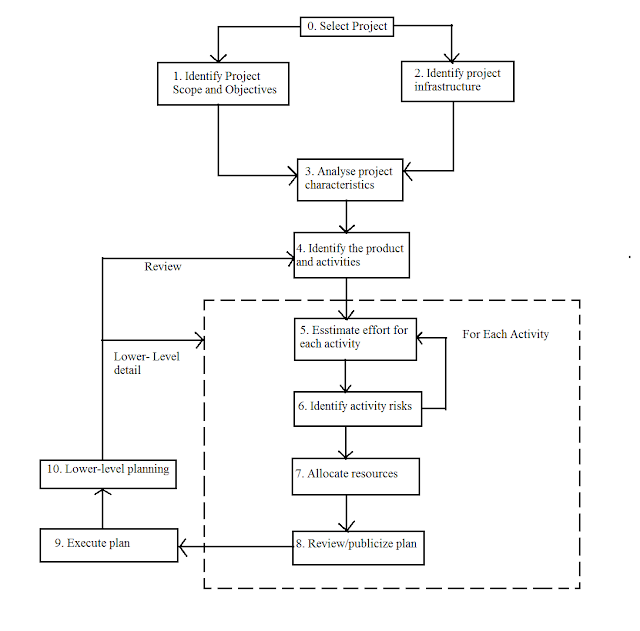
\includegraphics[width=\textwidth]{step_wise.png}
    \caption{Step Wise}
    \label{fig:3.1}
\end{figure}


%---------------------------------------------------
% Seccion 4
%---------------------------------------------------
\newpage
\section[Aproximación a la selección de proyecto apropiada]{Aproximación a la selección de\\proyecto apropiada}
\label{4.0.0}


%---------------------------------------------------
% Seccion 5
%---------------------------------------------------
\newpage
\section{Estimación del esfuerzo en Software}
\label{5.0.0}


%---------------------------------------------------
% Seccion 6
%---------------------------------------------------
\newpage
\section{Planificación de actividades}
\label{6.0.0}


%---------------------------------------------------
% Seccion 7
%---------------------------------------------------
\newpage
\section{Gestión del riesgo}
\label{7.0.0}

\subsection{Introducción}
\label{7.1.0}

{En esta sección se verá qué es un riesgo, cómo identificarlo y cómo gestionarlo mediante planificación.}

\subsection{Riesgo}
\label{7.2.0}

{Según PM-BOK (Guía de los fundamentos para la dirección de proyectos), un riesgo es <<un evento incierto o condición que, de cumplirse, tiene un efecto positivo o negativo en los objetivos de un proyecto>>.} \bigskip

{Según PRINCE2, un riesgo es <<la posibilidad de exposición a las consecuencias adversas de eventos futuros>>.} \bigskip

{Un riesgo tiene dos puntos fundamentales: \textbf{está relacionado con el futuro} (a elementos previsibles o, a veces, a cosas obviadas) e \textbf{implica causa y efecto} (y hay que tener en cuenta ambos).} \bigskip

{La gestión de riesgos se lleva a cabo principalmente en los puntos 3 y 6 del \nameref{fig:3.1} (\hyperref[fig:3.1]{figura 3.1}). Al estar los planes basados en suposiciones, la gestión de riesgos se ocupa de planificar en caso de que estas suposiciones sean incorrectas.}

\subsection{Categorías de riesgos}
\label{7.3.0}

{Para categorizar los riesgos, se utilizan las categorías usadas por Lyytinen, Mathiassen y Ropponen, que plantean estas 4:}

\begin{itemize}
    \item {\textbf{Actores}: riesgos que implican a las personas que rodean al proyecto.}
    \item {\textbf{Tecnología}: riesgos sobre la tecnología usada en el proyecto.}
    \item {\textbf{Estructura}: riesgos contenidos en el sistema y forma de gestión del proyecto.}
    \item {\textbf{Tareas}: riesgos acerca de las tareas del proyecto.}
\end{itemize}

\begin{figure} [ht]
    \centering
    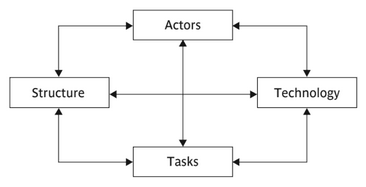
\includegraphics[keepaspectratio=true, scale=1.25]{images/Lyytinen-Mathiassen-Ropponen.png}
    \caption{Marco de riesgos Lyytinen-Mathiassen-Ropponen}
    \label{fig:7.1}
\end{figure}

\newpage
\subsection{Un marco para tratar riesgos}
\label{7.4.0}

{Los riesgos se gestionan de la siguiente manera (se amplia en las siguientes secciones):}

\begin{enumerate}
    \item {Identificación de riesgos}
    \item {Análisis y priorización de riesgos}
    \item {Planificación de riesgos}
    \item {Monitorización de riesgos}
\end{enumerate}

{Los 3 primeros se repiten para encontrar varios riesgos. Si se encuentra alguno que pueda intervenir en el éxito de un proyecto, se crean planes para reducirlo o eliminarlo.}

\subsection{Identificación de riesgos}
\label{7.5.0}

{Una opción es el \textbf{brainstorming}, donde los stakeholders se juntan y plantean posibles riesgos en común.} \bigskip

{Otra es la identificación casual o \textbf{casual mapping}, que consiste sencillamente en darse cuenta de qué puede afectar al proyecto.} \bigskip

{Otra es usar \textbf{checklists} o listas de riesgos ya existentes, ya sean de la compañía o de gente que haya hecho estudios, como el de Barry Bohem (1989).}

\newpage
{Según Barry Boehm, los 10 riesgos más comunes (en orden) son:}

\begin{enumerate}
    \item {\textbf{Falta de personal}: se reduce, por ejemplo, con una contratación de grandes talentos.}
    \item {\textbf{Estimación de tiempo y costes poco realistas}: se reduce, por ejemplo, aplicando múltiples técnicas de estimación.}
    \item {\textbf{Desarrollo de las funciones Software erróneas}: se reduce, por ejemplo, mediante prototipado.}
    \item {\textbf{Desarrollo de las interfaces de usuario erróneas}: se reduce, por ejemplo, mediante prototipado.}
    \item {\textbf{Chapado en oro}: se reduce, por ejemplo, mediante un análisis de coste-beneficio.}
    \item {\textbf{Cambios tardíos en los requisitos}: se reduce, por ejemplo, mediante procedimientos estrictos de control de cambios.}
    \item {\textbf{Déficit de componentes suministrados externamente}: se reduce, por ejemplo, mediante una formalización de especificaciones.}
    \item {\textbf{Deficiencias en las tareas realizadas externamente}: se reduce, por ejemplo, procedimientos de garantía de calidad.}
    \item {\textbf{Deficiencias de rendimiento en tiempo real}: se reduce, por ejemplo, mediante simulaciones.}
    \item {\textbf{Desarrollo técnico demasiado difícil}: se reduce, por ejemplo, mediante análisis técnicos.}
\end{enumerate}

\subsection{Evaluación de riesgos}
\label{7.6.0}

{Una forma de evaluar los riesgos es calculando la \textbf{exposición al riesgo}, una unidad monetaria que se calcula de la siguiente manera:}

\begin{equation}
    \text{exposición al riesgo} = \text{daño potencial} \times \text{probabilidad del suceso}
\end{equation}

{Sin embargo, no todos los riesgos pueden ser medidos en unidades monetarias. También puede haber casos en los que el riesgo se mida en esfuerzo o tiempo. Ocurre también que muchos managers están en contra de cálculos tan precisos, y prefieren utilizar para el daño potencial y para la probabilidad del suceso escalas del 1 al 10, quedando la exposición en una escala del 1 al 100.} \bigskip

{Sea cual sea el cálculo, Boehm recomienda centrarse en los 10 riesgos con más exposición. Si el proyecto es pequeño, se puede centrar en una cantidad menor.}

\newpage
{A veces se hacen cálculos cualitativos para las dos variables de cálculo, siendo los valores posibles <<alto>>, <<significativo>>, <<moderado>> o <<bajo>>:}

% Please add the following required packages to your document preamble:
% \usepackage{booktabs}
% \usepackage{graphicx}
\begin{table}[ht]
\centering
\resizebox{\textwidth}{!}{%
\begin{tabular}{@{}lll@{}}
              & Daño potencial          & Probabilidad del suceso       \\ \hline
Alto          & Mayor de 30\%           & Mayor de 50\%                 \\
Significativo & 20-30\%                 & 30-50\%                       \\
Moderado      & 10-19\%                 & 10-29\%                       \\
Bajo          & Menos del 10\%          & Menos del 10\%                \\ \hline
              & Del gasto presupuestado & De probabilidad de que ocurra
\end{tabular}%
}
\caption{Descriptores cualitativos}
\label{tab:7.1}
\end{table}

{De esta manera se pueden situar los riesgos en una matriz y establecer una línea de tolerancia, por debajo de la cual no se considerarán los riesgos, y por encima de la cual se escogerán los 10 riesgos con mayor exposición:}

\begin{figure} [ht]
    \centering
    \includegraphics[keepaspectratio=true, scale=1.00]{images/Matriz de exposición de riesgo.png}
    \caption{Matriz de exposición al riesgo}
    \label{fig:7.2}
\end{figure}

\newpage
\subsection{Planificación de riesgos}
\label{7.7.0}

{Existen 5 estrategias principales de lidiar con riesgos:}

\subsubsection{Aceptación del riesgo}
\label{7.7.1}

{El riesgo es menos costoso que el coste de cualquier mitigación. No se hace nada al respecto.}

\subsubsection{\textit{Evitación} del riesgo}
\label{7.7.2}

{No se realiza la tarea que conlleva el riesgo, y así no existe la probabilidad de este riesgo.}

\subsubsection{Reducción del riesgo}
\label{7.7.3}

{Se toman acciones que reducen la probabilidad del riesgo.}

\subsubsection{Mitigación del riesgo}
\label{7.7.4}

{Se toman acciones que mitigan el daño del riesgo.}

\subsubsection{Transferencia del riesgo}
\label{7.7.5}

{La tarea que genera el riesgo es transferida a otra persona u organización.}

\subsection{Gestión de riesgos}
\label{7.8.0}

\subsubsection{Contingencia}
\label{7.8.1}

{Un plan de contingencia es aquel que se lleva a cabo si un riesgo se materializa. Este puede conllevar unos costes de preparación y otros de realización.}

\subsubsection{Decidiendo las acciones para cada riesgo}
\label{7.8.2}

{Todas las contramedidas llevadas a cabo deben ser rentables. Para medir esta rentabilidad, se usa la fórmula del \textbf{nivelado de la reducción de riesgo} (risk reduction leverage):}

\begin{equation}
    \text{nivelado de la reducción de riesgo} = \frac{\text{RE}_\text{antes} - \text{RE}_\text{después}}{\text{coste de la reducción de riesgo}}
\end{equation}

{Donde cada \textit{RE} es cada exposición al riesgo (\textit{Risk Exposure}) antes y después de la acción de reducción. Cualquier valor por encima de $1.00$ significa que la acción merece la pena.}

\subsubsection{Crear y mantener un riesgo}
\label{7.8.3}

{Los riesgos se van anotando en registros que regularmente se revisan, actualizan en caso de cambios y corrigen. Si se establecen como <<cerrados>>, no se vuelven a revisar.}

\subsection{Evaluación de riesgos para planificar}
\label{7.9.0}

{Desde aquí se asume que el riesgo es o tiene como resultado que una tarea termine más tarde de lo planificado. En estos casos, muchas veces se asume o espera que se compense el tiempo extra con tiempo de menos que tarde otra tarea. Sin embargo, los desarrolladores tienden a utilizar todo el tiempo ofrecido para la tarea (ley de Parkinson).}

\subsection{Aplicando PERT}
\label{7.10.0}

\subsubsection{Usando PERT para evaluar los efectos de la incertidumbre}
\label{7.10.1}

{PERT se utiliza para tener en cuenta la incertidumbre en las estimaciones de las duraciones de las tareas. Por ello, utiliza estas variables:}

\begin{itemize}
    \item {\textbf{Tiempo más probable} \textit{m}: el tiempo que se tardaría en realizar la tarea en circunstancias normales.}
    \item {\textbf{Tiempo optimista} \textit{a}: el tiempo que menos se podría tardar en realizar la tarea.}
    \item {\textbf{Tiempo pesimista} \textit{b}: el tiempo que más podría llevar la tarea.}
\end{itemize}

{Con esto, PERT ofrece una fórmula para la \textbf{duración esperada}:}

\begin{equation}
    t_e = \frac{a + 4m + b}{6}
\end{equation}

\subsubsection{Usando las duraciones esperadas}
\label{7.10.2}

{PERT ofrece dos cosas: la \textbf{fecha esperada de finalización} y la \textbf{duración esperada de cada tarea}. Es importante remarcar que en ambos casos es lo esperado, ya que tiene en cuenta la incertidumbre.}

\subsubsection{Desviación estándar de las actividades}
\label{7.10.3}

{La desviación estándar da el grado de incertidumbre de la duración estimada. Su fórmula es:}

\begin{equation}
    s = \frac{b - a}{6}
\end{equation}

\subsubsection{Probabilidad de cumplir objetivos}
\label{7.10.4}

{PERT ofrece un método de cálculo de probabilidades de cumplir objetivos para cada tarea utilizando el z-valor y convirtiéndolo en una probabilidad (el libro no da muchos más detalles):}

\begin{enumerate}
    \item Se calcula la desviación estándar de cada evento.
    \item Se calcula el z-valor para cada evento que tenga una fecha objetivo.
    \item se convierte el z-valor en una probabilidad.
\end{enumerate}

\subsubsection{Cálculo de desviaciones para cada evento}
\label{7.10.5}

\begin{itemize}
    \item {Para el tiempo en una cadena de eventos, se calcula la suma de tiempos de dichos eventos. Por ejemplo: $t_1 + t_2 + t_3$...}
    \item {En caso de que haya varias formas de llegar al mismo evento, el tiempo final será el mayor de los valores. Por ejemplo, en \nameref{fig:7.3}, se puede llegar al nodo 5 a través de 1-3-5 o a través de 1-5, pero se coge el valor de 1-5 al ser mayor.}
    \item {Para la desviación estándar en una cadena de eventos, se calcula la raíz cuadrada de la suma de los cuadrados. Por ejemplo: $\sqrt{s_1^2 + s_2^2 + s_3^2}$.}
    \item {De nuevo, en caso de que haya varias formas de llegar al mismo evento, la desviación será el mayor de los valores. Por ejemplo, en \nameref{fig:7.3}, se escogería también el camino 1-5, al ofrecer el mayor de las desviaciones.}
\end{itemize}

\begin{figure} [ht]
    \centering
    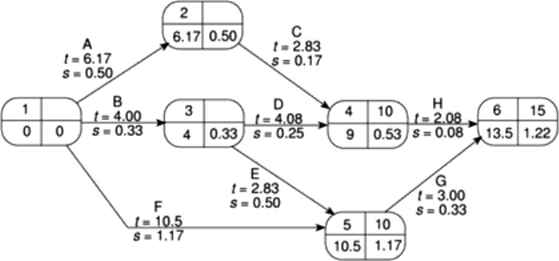
\includegraphics[keepaspectratio=true, scale=0.80]{images/Red_PERT.jpg}
    \caption{Ejemplo de red PERT}
    \label{fig:7.3}
\end{figure}

\subsubsection{Cálculo del z-valor}
\label{7.10.6}

\begin{equation}
    z = \frac{T - t_e}{s}
\end{equation}

{Donde $T$ es la fecha objetivo, $t_e$ es el valor esperado y $s$ es la desviación. El z-valor puede dar valores negativos, y estos dan la mayor probabilidad de \textbf{no} cumplir la fecha objetivo (la fecha real va atrasada).}

\subsubsection{Ventajas de PERT}
\label{7.10.7}

{PERT se centra en la incertidumbre de las previsiones y permite establecer un ránking de las tareas con mayor incertidumbre para vigilarlas más de cerca.}

\newpage
\subsection{Simulación de Montecarlo}
\label{7.11.0}

{La simulación de Montecarlo es una simulación realizada por ordenador que es capaz de calcular infinitas posibilidades a partir de una serie de variables. Se utiliza para trabajos de investigación, pero también vale para calcular el riesgo de no cumplir los objetivos.}

\subsection{Concepto de cadena crítica}
\label{7.12.0}

{Generalmente, se espera que las finalizaciones tempranas de tareas ofrezcan tiempo extra al proyecto. Sin embargo, por la ley de Parkinson, se sabe que por lo general esto no va a ocurrir.} \bigskip

{La \textbf{cadena crítica} es la cadena de actividades más larga del proyecto, teniendo en cuenta dependencias de tareas y recursos. Es importante \textbf{no confundirla con el camino crítico}, que solo tiene en cuenta dependencias de tareas.}

\subsubsection{Derivación de la duración de las tareas <<más probables>>}
\label{7.12.1}

{La planificación de cadenas críticas suele situar la fecha objetivo de una de estas como aquella con un 50\% de probabilidades de tener éxito. Algunos gestores suelen dividir a la mitad el tiempo estimado o reducirlo un 33\%, dado que esto suele ofrecer más probabilidades de terminar a tiempo la cadena. Sin embargo, esto desmotiva a los trabajadores.}

\subsubsection{Uso de los inicios más tardíos para actividades}
\label{7.12.2}

{A veces se retrasa los proyectos hasta su inicio más tardío para que no se pueda añadir a sus trabajadores a otros proyectos. Otros argumentan que son los trabajadores los que tienden a empezar en el inicio más tardío.}

\subsubsection{Insertando \textit{buffers} de proyecto y de alimentación}
\label{7.12.3}

{Para lidiar con sobrepasos de tiempo, a veces se reduce a la mitad todas las zonas de confort de la cadena crítica y se juntan en un solo tiempo al final del proyecto llamado \textbf{\textit{buffer} de proyecto}. Así, si una actividad de la cadena crítica retrasa el proyecto, este se aplazará dentro del \textit{buffer} del proyecto.} \bigskip

{Otra forma de calcular el \textit{buffer} de proyecto es mediante la raíz cuadrada de la suma de los cuadrados de las zonas de confort ($\sqrt{t_1^2 + t_2^2 + t_3^2...}$), basado en las desviaciones típicas. Este cálculo tiene en cuenta la compensación de la duración de las tareas (las terminadas pronto compensa las terminadas tarde).} \bigskip

{El \textbf{\textit{buffer} de alimentación} trata de hacer lo mismo que el de proyecto pero con cadenas de tareas que no pertenezcan a la cadena crítica (cadenas de alimentación). Se suelen colocar donde la cadena de alimentación se una a la cadena crítica y se calcula igual que el \textit{buffer} de proyecto.}

\newpage
\subsubsection{Ejecución del proyecto}
\label{7.12.4}

{Puntos clave al ejecutar el proyecto:}

\begin{itemize}
    \item {Las cadenas de tareas no deben comenzarse antes de tiempo, pero una vez comenzadas deben terminar lo antes posible.}
    \item {Los \textit{buffers} se dividen en 3 zonas iguales:}
    
    \begin{itemize}
        \item {\textbf{verde}: no hay que aplicar ninguna estrategia.}
        \item {\textbf{ámbar}: conviene formular un plan de acción.}
        \item {\textbf{rojo}: se ejecuta el plan de acción.}
    \end{itemize}
\end{itemize}

{A la planificación de cadenas críticas se le puede sumar dos conceptos complementarios que aseguren la gestión del proyecto:}

\begin{itemize}
    \item {\textbf{El cálculo de dos estimaciones}: la duración más probable y la duración segura (tiempo que se tarda en resolver los problemas y en finalizar la tarea).}
    \item {\textbf{Colocar tiempos de contingencia} (que viene de calcular la duración segura menos la duración más probable) en un \textit{buffer} en lugar de asignarlos a cada actividad.}
\end{itemize}


%---------------------------------------------------
% Seccion 8
%---------------------------------------------------
\newpage
\section{Asignación de recursos}
\label{8.0.0}

\subsection{Introducción}
\label{8.1.0}

{Durante la asignación de recursos (figura~\ref{fig:3.1}: \nameref{fig:3.1}, paso 7), se pretende enlazar los recursos disponibles con el plan de actividades, cambiando este último de ser necesario para ajustarse a los recursos. El resultado final de la asignación de recursos será:}

\begin{itemize}
    \item {El esquema de actividades.}
    \item {Un esquema de recursos que muestre cuándo y dónde se utiliza cada recurso.}
    \item {Un esquema de costes que muestre el gasto acumulado por recurso y tiempo.}
\end{itemize}

\subsection{La naturaleza de los recursos}
\label{8.2.0}

{Un recurso es un elemento o persona requerida para la ejecución de un proyecto. Los recursos se clasifican en 7 categorías:}

\begin{itemize}
    \item {\textbf{Laboral}: aquí pertenecen los trabajadores, tanto desarrolladores como otros equipos o incluso clientes que estén involucrados en el proyecto.}
    \item {\textbf{Equipamiento}: estaciones de trabajo, equipo de oficina, ordenadores, sillas, mesas...}
    \item {\textbf{Materiales}: elementos que serán <<consumidos>> para llevar a cabo el proyecto (CD's donde se graba el Software a vender, hardware, etc.).}
    \item {\textbf{Espacio}: oficinas, despachos, salas de reuniones...}
    \item {\textbf{Servicios}: en algunos proyectos se necesitan servicios especializados (alquiler y manutención de dominios, servicios de telecomunicaciones, etc.).}
    \item {\textbf{Tiempo}: recurso que se pretende reducir mediante el uso del resto de recursos.}
    \item {\textbf{Dinero}: recurso secundario usado para conseguir recursos y consumido por el uso de los mismos.}
\end{itemize}

\subsection{Identificación de recursos necesarios}
\label{8.3.0}

{El primer paso para la asignación de recursos es repasar las actividades del proyecto y listar qué recurso necesita cada actividad. Algunos recursos no serán específicos de actividades sino de la infraestructura del proyecto o incluso habrá recursos que se necesiten para apoyar otros recursos.}

\newpage
\subsection{Planificación de recursos}
\label{8.4.0}

{Una vez se tienen listados los recursos necesarios, hay que enlazar esta lista con la de tareas para distribuir los recursos. Esto se puede ver en el ejemplo del libro (figura~\ref{fig:8.1}: \nameref{fig:8.1}).}

\begin{figure} [ht]
    \centering
    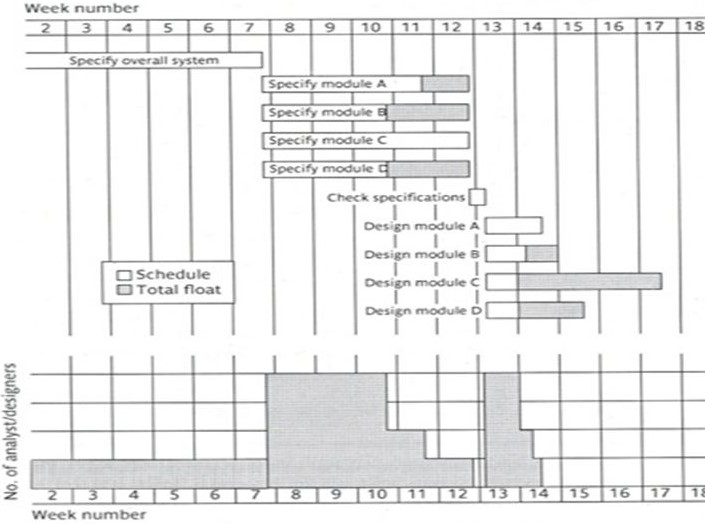
\includegraphics[keepaspectratio=true, scale=0.50]{images/Histograma_y_actividades.jpg}
    \caption{Ejemplo de histograma de recursos}
    \label{fig:8.1}
\end{figure}

{Cambiar la cantidad de recursos durante el tiempo también añade costes al proyecto. Conviene mantener los mismos recursos durante el proyecto y evitar sobrecargas sobre recursos. Esto se ve representado en el histograma: si existen picos o valles en el histograma, es que se están aprovechando mal los recursos (cada fila es un recurso distinto). Un histograma perfecto debe ser liso (o suave, la traducción es ambigua), lo que implicaría una repartición correcta de los recursos.}

\begin{figure} [ht]
    \centering
    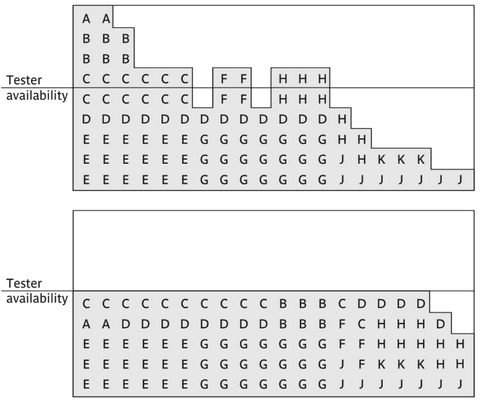
\includegraphics[keepaspectratio=true, scale=0.75]{images/Suavizado_de_histograma.png}
    \caption{Histograma alisado}
    \label{fig:8.2}
\end{figure}

\newpage
{Para lograr el alisado, se pueden atrasar las fechas de inicio de algunas actividades (que tengan zona de confort) o incluso dividirlas en partes, aunque en proyectos de software, no siempre es posible dividir actividades sin aumentar el tiempo que llevan. Otra técnica usada para lograr el alisado es que, actividades que necesiten varios trabajadores, utilicen un solo recurso y aumente su duración (así se evita acumular trabajadores en una sola tarea).} \bigskip

{En caso de que no se consiga alisar el histograma, resulta muy útil priorizar actividades. Casi siempre se va a priorizar aquella actividad que esté en el camino crítico. Existen dos estrategias útiles:}

\begin{itemize}
    \item {\textbf{Prioridad por flotabilidad total}: a menos flotabilidad, más prioridad. Es recomendable recalcular las flotabilidades cada vez que se retrase un proyecto.}
    \item {\textbf{Prioridad por lista ordenada}: se basa en ordenarlas según criterios como el de la lista de prioridades de \textbf{Burman}:}
    
    \begin{enumerate}
        \item \textbf{Actividad crítica más corta}
        \item \textbf{Actividad crítica}
        \item \textbf{Actividad no crítica más corta}
        \item \textbf{Actividad no crítica con menos flotabilidad}
        \item \textbf{Actividad no crítica}
    \end{enumerate}
    
\end{itemize}

{Si aún así no se puede alisar el histograma, hay que considerar ampliar los recursos o cambiar los métodos de trabajo.}

\subsection{Creación de caminos críticos}
\label{8.5.0}

{Al asignar recursos y/o alisar el histograma se pueden generar nuevos caminos críticos. La técnica comentada en la sección~\ref{8.4.0} de atrasar fechas de inicio puede crear actividades críticas si consume toda la flotabilidad. También puede ocurrir que se retrase la disponibilidad de un recurso si este se retrasa en una tarea.}

\subsection{Cálculo del coste}
\label{8.6.0}

{Algunas acciones durante el asignado de recursos acarrearán costes. Habrá que considerar si estos son más baratos que retrasar la entrega del proyecto o que no cumplir las fechas.}

\subsection{Siendo específicos}
\label{8.7.0}

{En los proyectos de software, la experiencia individual de cada miembro cuenta para el proyecto. Asignar pronto al personal nos puede ayudar a reestimar mejor la duración de las actividades según su habilidad.}

\newpage
{Algunos factores a tener en cuenta en cuanto a la asignación de personal específico:}

\begin{itemize}
    \item {\textbf{Disponibilidad}: es necesario saber la disponibilidad de cada empleado.}
    \item {\textbf{Criticidad}: los empleados más experimentados pueden reducir la duración del proyecto.}
    \item {\textbf{Riesgo}: los empleados más experimentados pueden reducir la incertidumbre de las actividades que impliquen más riesgo.}
    \item {\textbf{Entrenamiento}: las actividades menos críticas pueden ser llevadas a cabo por los empleados menos experimentados y pueden ayudarles a desarrollar habilidades. También son más baratos.}
    \item {\textbf{Team building}: la selección según sus perfiles puede ser útil para mejorar la colaboración del equipo (capítulo~\ref{12.0.0}).}
\end{itemize}

\subsection{Publicación de la planificación de recursos}
\label{8.8.0}

{Las planificaciones de recursos se suelen publicar como en la figura~\ref{fig:8.3}. Estas no cuentan con días no productivos (días festivos, vacaciones, bajas, etc.). Después de esta publicación se transfiere la información a la red de precedencia para corregir la planificación de actividades.}

\begin{figure} [ht]
    \centering
    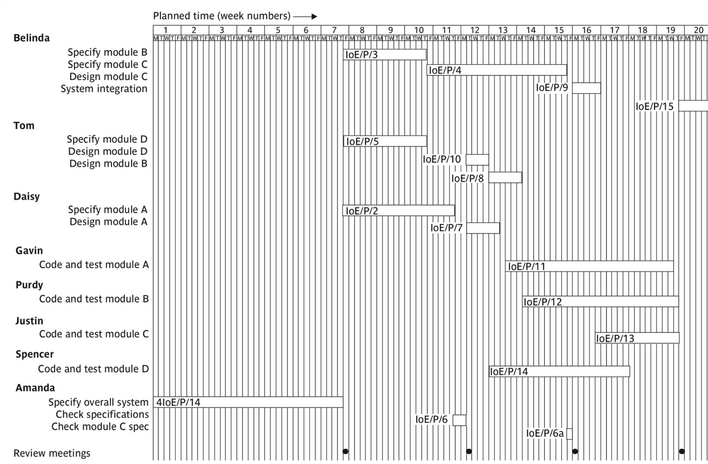
\includegraphics[keepaspectratio=true, scale=0.75]{images/plan_de_recursos.png}
    \caption{Planificación de recursos}
    \label{fig:8.3}
\end{figure}

\newpage
\subsection{Planificación de costes}
\label{8.9.0}

{Se realiza un desglose detallado de costes clasificado por:}

\begin{itemize}
    \item {\textbf{Costes de personal}: salarios y costes directos de contratación.}
    \item {\textbf{Gastos de administración}: gastos generales de la empresa que no pueden ser directamente relacionados con el proyecto.}
    \item {\textbf{Cargos por uso}: costes que tengan una relación directa con el uso.}
\end{itemize}

\subsection{Secuencia de planificado}
\label{8.10.0}

{Cualquier cambio al plan de actividades afectará al de asignación de recursos y viceversa, e igualmente afectará un cambio en cualquiera de estos dos en la evaluación de riesgos y en la planificación de costes. Una buena planificación de proyectos será capaz de demostrar los cambios que generará cada cambio y de mantener una buena sincronía entre todos estos esquemas. La experiencia y habilidad del gestor de proyectos también serán de gran utilidad.}

%---------------------------------------------------
% Seccion 9
%---------------------------------------------------
\newpage
\section{Monitorización y control}
\label{9.0.0}

\subsection{Introducción}
\label{9.1.0}

{Una vez comienza el proyecto, se debe recoger información sobre los avances para compararlos con la planificación. Aquí se tratará cómo se recoge la información y qué decisiones tomar para cumplir con las fechas.}

\subsection{Creación del marco de trabajo}
\label{9.2.0}

{La monitorización hay que ejecutarla de manera regular para encontrar qué ocurre y compararlo con los objetivos. Si no se están cumpliendo, hay que replantear la planificación o, en algunos casos, replantear los objetivos.} \bigskip

{Generalmente, al monitorizar se vigilan \textbf{atrasos} en fechas de objetivos, déficits de \textbf{calidad}, \textbf{funcionalidad no adecuada} y \textbf{sobrecostes}.}

\subsubsection{Responsabilidad}
\label{9.2.1}

{La responsabilidad general de asegurar un progreso satisfactorio en el proyecto es del \textbf{comité de dirección de proyecto} (\textit{project steering comittee}). La diaria recae en el \textbf{director del proyecto} y, salvo en los proyectos más pequeños que tienen un solo equipo por proyecto, algunos aspectos pueden delegarse en los \textbf{jefes de equipo}.} \bigskip

{Los informes se realizan de manera regular y ascendente en la jerarquía de manera oral o escrita, formal o informal y periódico o ad hoc.}

\subsubsection{Evaluación del progreso}
\label{9.2.2}

{La información debe ser objetiva y tangible siempre que se pueda. A veces la información estará basada en tareas parcialmente completadas.}

\subsubsection{Estableciendo puntos de control}
\label{9.2.3}

{Habrá puntos de control periódicos (mensuales por ejemplo) o atados a eventos del proyecto.}

\subsubsection{Tomando \textit{snapshots}}
\label{9.2.4}

{La frecuencia de los informes dependerá del tamaño y riesgo del proyecto. Además, a mayor rango en jerarquía, menor frecuencia y detalle tendrán estos informes. A nivel de desarrollador, sin embargo, se aconseja que sea \textbf{semanal}. A niveles superiores (información al comité de dirección de proyecto), los informes suelen enviarse en puntos particulares de la vida del proyecto conocidos como \textbf{puntos de control} o puntos de revisión.}

\subsection{Recogiendo información}
\label{9.3.0}

{Es necesario recoger información tanto de tareas completas como parcialmente completas (y cuánto puede quedar). Para estimar cuánto queda para estas, a veces se usan \textit{productos intermedios} (como la primera compilación, por ejemplo) para determinar el avance.}

\subsubsection{Informes de finalización parcial}
\label{9.3.1}

{Para determinar el tiempo trabajado en una tarea y poder estimar el tiempo restante, se suelen usar las fichas de tiempo (\textit{time sheets}), donde el empleado apunta el tiempo (generalmente en horas) que ha dedicado a cada actividad durante la semana completa.}

\subsubsection{Informes RAG (\textit{Red}/\textit{Amber}/\textit{Green})}
\label{9.3.2}

{Para evitar preguntar por las fechas de compleción estimadas para una actividad, a veces se usa la estimación \textbf{RAG}, una estimación cualitativa basada en semáforos que consiste en dividir una actividad en tareas, señalarlas con estos tres colores para determinar si <<entra en la fecha objetivo>> (verde), <<no entra pero es recuperable>> (ámbar) o <<no entra y dificilmente se puede recuperar>> (rojo) y estimar a partir de estos una evaluación general para la actividad.}

\subsection{Visualización del progreso}
\label{9.4.0}

\subsubsection{Diagrama de Gantt}
\label{9.4.1}

{El diagrama de Gantt muestra mediante barras de actividades la fecha programada para la actividad, la duración (a menudo junto con la flotabilidad) y el progreso (coloreando la barra hasta donde se estima que está completado).}

\begin{figure} [ht]
    \centering
    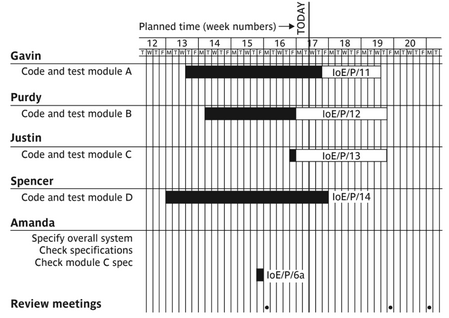
\includegraphics[keepaspectratio=true, scale=0.75]{images/Gantt.png}
    \caption{Diagrama de Gantt}
    \label{fig:9.1}
\end{figure}

\subsubsection{Diagrama de deslizamiento o \textit{slip chart}}
\label{9.4.2}

{Igual que el diagrama de Gantt pero la línea que indica la fecha actual se <<tuerce>> hacia el punto de compleción de cada tarea. Una barra muy torcida indica la necesidad de replanificación.}

\begin{figure} [ht]
    \centering
    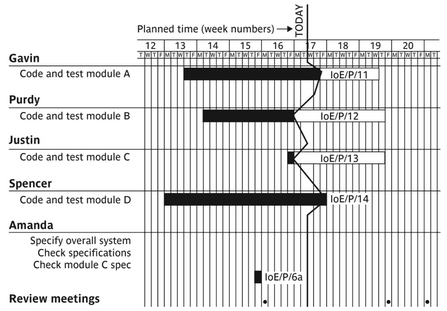
\includegraphics[keepaspectratio=true, scale=0.75]{images/slip_chart.png}
    \caption{\textit{Slip chart}}
    \label{fig:9.2}
\end{figure}

\subsubsection{Cronograma o \textit{timeline}}
\label{9.4.3}

{Muestra de manera gráfica la variación en las fechas objetivo durante la vida del proyecto. Las líneas que bajan indican el avance de cada tarea hasta que tocan la diagonal, que es la fecha donde terminan. Su evaluación tras la finalización del proyecto puede delatar fallos en el proceso de estimación.}

\begin{figure} [ht]
    \centering
    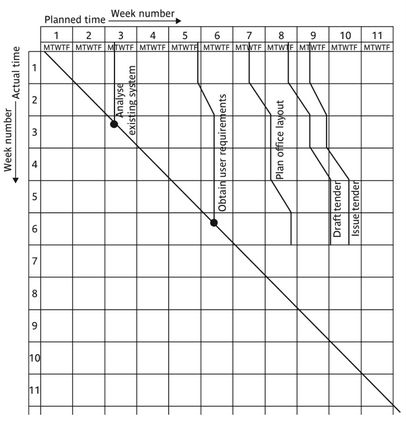
\includegraphics[keepaspectratio=true, scale=0.75]{images/timeline_chart.png}
    \caption{\textit{Timeline}}
    \label{fig:9.3}
\end{figure}

\subsection{Monitorización de costes}
\label{9.5.0}

{Mediante un diagrama de gastos acumulativos se puede ver la diferencia entre los gastos planeados y los reales. Puede indicar si un proyecto va atrasado (sus costes son menores que los planeados). A la línea de gasto real se le puede añadir el gasto esperado (basado en las actividades sin completar) para estimar una fecha de finalización de proyecto revisada.}

\subsection{Análisis del valor ganado (\textit{Earned Value})}
\label{9.6.0}

{A cada tarea del proyecto, se le asigna un valor basado en la estimación original de gastos. A este se le llama \textbf{\textit{Planned Value}} (PV) o \textbf{\textit{Budgeted Cost of Work Scheduled}} (BCWS). Una tarea sin comenzar tiene un \textbf{\textit{Earned Value}} (EV) o \textbf{\textit{Budgeted Cost of Work Performed}} (BCWP) de cero, y cuando se completa su EV es igual a su PV.} \bigskip

{Cuando una tarea esta a medias y no hay forma exacta de determinar el porcentaje que se ha completado, se determina su EV de distintas maneras:}

\begin{itemize}
    \item \textbf{0/100}: la tarea vale el 0\% de su PV cuando se comienza y el 100\% cuando se termina.
    \item \textbf{50/50}: la tarea vale el 50\% de su PV cuando se comienza y suma el 50\% restante cuando se termina.
    \item \textbf{75/25}: la tarea vale el 75\% de su PV cuando se comienza y suma el 25\% restante cuando se termina.
    \item \textbf{Técnica del milestone}: la tarea recibe su valor basado en los hitos que se completen.
    \item \textbf{Porcentaje completo}: la tarea se puede medir objetivamente y se calcula su porcentaje.
\end{itemize}

{Se recomienda usar la técnica 0/100 en todos los casos en que no se pueda medir el avance.}

\subsubsection{Presupuesto base}
\label{9.6.1}

{El presupuesto base (baseline) es el gasto planteado en el plan de proyecto inicial y muestra el PV a través del tiempo (muchas veces medido en horas/hombre).}

\subsubsection{Monitorizando el EV}
\label{9.6.2}

{Una vez dibujado el presupuesto base, se va dibujando el progreso del EV por días según se completen las tareas. También se va grabando el \textbf{\textit{Actual Cost}} (AC) o coste real, también llamado \textbf{\textit{Actual Cost of Work Performed}} (ACWP).}

\subsubsection{Desviación del programa o \textit{Schedule Variance} (SV)}
\label{9.6.3}

{La desviación del programa se calcula como $SV = EV - PV$. Muestra la desviación del valor planeado en una fecha concreta.}

\subsubsection{Desviación del tiempo o \textit{Time Variance} (TV)}
\label{9.6.4}

{Si $T_p$ es la fecha en la que se planeaba conseguir un PV concreto y $T_a$ la fecha en la que se consigue ese valor como EV, $TV$ se calcula como $TV = T_a - T_p$. Muestra la diferencia de tiempo en conseguir un valor concreto. Si es negativo, significa que se está tardando más de lo planeado.}

\subsubsection{Desviación de coste o \textit{Cost Variance} (CV)}
\label{9.6.5}

{La desviación de coste se calcula como $CV = EV - AC$. Muestra la diferencia entre el valor ganado hasta un punto del proyecto y el coste real para conseguir dicho avance en ese punto.}

\subsubsection{Ratios de rendimiento}
\label{9.6.6}

{Existen dos importantes:}

\begin{itemize}
    \item {\textbf{\textit{Cost Performance Index}} o índice de rendimiento de costes}
    \begin{itemize}
        \item $CPI=EV/AC$
        \item da un ratio relacionado con el Cost Variance
    \end{itemize}
    
    \item {y el \textbf{\textit{Schedule Performance Index}} o índice de rendimiento de programa }
    \begin{itemize}
        \item $SPI=EV/PV$
        \item da un ratio relacionado con el Schedule Variance
    \end{itemize}
\end{itemize}

{Ambos ratios son favorables si dan un valor mayor que 1.}

\subsection{Prioridades de monitorización}
\label{9.7.0}

{Al monitorizar hay que prestar atención siguiendo este orden:}

\begin{enumerate}
    \item {\textbf{Actividades del camino crítico}.}
    \item {\textbf{Actividades sin flotabilidad}.}
    \item {\textbf{Actividades con flotabilidad menor} a una especificada por el director de proyectos.}
    \item {\textbf{Actividades con alto riesgo}.}
    \item {\textbf{Actividades que usen recursos críticos}.}
\end{enumerate}

\subsection{Devolviendo el proyecto a su fecha objetivo}
\label{9.8.0}

{Si ocurren eventos inesperados o retrasos, el director de proyecto debe reorganizar las tareas del proyecto asegurando (o intentando) que la fecha objetivo permanezca intacta. Existen dos estrategias principales: \textbf{acortar el camino crítico} y \textbf{modificar los requisitos de precedencia} de actividades.}

\subsubsection{Acortar el camino crítico}
\label{9.8.1}

{Estrategias posibles:}

\begin{itemize}
    \item {Añadir recursos (especialmente personal)}
    \item {Incrementar el uso de los recursos actuales}
    \item {Reasignar personal al camino crítico}
    \item {Reducir el alcance (eliminando funcionalidades)}
    \item {Reducir la calidad}
\end{itemize}

{Acortar el camino crítico a veces causa que otros caminos se vuelvan críticos.}

\subsubsection{Reconsiderar los requisitos de precedencia}
\label{9.8.2}

{Se plantea hasta que punto algunas actividades necesitan esperar a que otras hayan terminado para ser iniciadas. También se plantea dividir actividades en sub-actividades donde alguna de ellas pueda iniciarse antes. Estas acciones pueden comprometer la calidad.}

\subsubsection{Conservación del \textit{Business Case}}
\label{9.8.3}

{La preocupación de los stakeholders será que se mantenga el \textit{Business Case}. Si este se altera, se podría cancelar el proyecto.}

\subsubsection{Planificación de excepciones}
\label{9.8.4}

{Normalmente se permite al director de proyecto cambiar la planificación mientras los resultados se generen a tiempo y dentro de lo presupuestado. Pero si los cambios afectan a las fechas de entrega, al alcance o a los costes, necesitarán la aprobación de los stakeholders. Para ello, el director de proyecto escribirá un \textbf{Informe de Excepción} (exception report) donde explicará las razones de la desviación del plan existente y detallará las consecuencias. Si el Comité Directivo del Proyecto aprueba el informe, el director de proyecto creará un informe detallado y, si el Comité lo aprueba, podrá ejecutar los cambios al plan.}

\subsection{Control de cambios}
\label{9.9.0}

{El documento de requisitos de usuario puede cambiar durante los ciclos de desarrollo y revisión del proyecto, pero llegado un punto se considera una versión final y se paraliza el documento. A partir de aquí, cualquier cambio del documento puede afectar al proyecto completo.}

\subsubsection{Rol de bibliotecario de configuraciones}
\label{9.9.1}

{El bibliotecario de configuraciones, bibliotecario del proyecto o gestor de configuraciones (en el libro lo describen cada vez de una manera) tiene varias responsabilidades con respecto al control de cambios:}

\begin{itemize}
    \item {Identifica todos los elementos sujetos al control de cambios.}
    \item {Mantiene un depósito central con las copias maestras de toda la documentación del proyecto y los productos generados.}
    \item {Establece un procedimiento formal para gestionar cambios.}
    \item {Mantiene registros de quién tiene acceso a qué artículos de la biblioteca y el estado de cada artículo de la biblioteca.}
\end{itemize}

\subsubsection{Procedimientos de control de cambios}
\label{9.9.2}

{Se siguen los siguientes pasos:}
\begin{enumerate}
    \item {Un usuario percibe un cambio necesario del sistema.}
    \item {La Gestión de Usuarios considera (y filtra) las solicitudes de cambio (\textbf{\textit{RFC}}, \textit{Request for Change}) de usuarios, buscando que el cambio genere un beneficio real. De ser así, se lo pasa a Gestión de Desarrollo.}
    \item {Una sola persona del area de desarrollo recibe y procesa la RFC. Se revisa la practicidad y costes del cambio y los productos afectados por el mismo.}
    \item {Se informa a la Gestión de Usuarios con los resultados y estos deciden si seguir adelante.}
    \item {Se priorizarán los RFC a llevar a cabo: el rol de Junta de Control de Cambios, formado por representantes de stakeholders, aceptará y priorizará cambios pequeños documentados en RFC's que no excedan costes ni fechas de entrega. Si el cambio es grande, o se acumulan muchos cambios pequeños, la responsabilidad ascenderá en la jerarquía.}
    \item {Se aprueba la ejecución de un RFC asignando desarrolladores que solicitarán al bibliotecario accesso a una copia maestra.}
    \item {Se modifica la copia.}
    \item {Se avisa a Gestión de Usuarios y se realizan pruebas de aceptación sobre copias de la versión.}
    \item {Una vez el usuario está satisfecho se autoriza la liberación de copias.}
\end{enumerate}

\subsubsection{Cambios en el alcance del sistema}
\label{9.9.3}

{El tamaño del sistema tiende a crecer con los cambios. Es necesario monitorizar esto.}

%---------------------------------------------------
% Seccion 10
%---------------------------------------------------
\newpage
\section{Gestión de contratos}
\label{10.0.0}

\subsection{Introducción}
\label{10.1.0}

{Este tema tratará sobre la contratación de recursos y servicios externos. Es necesario, en estos contratos, dejar claro desde el principio los requisitos y asegurarse de que los bienes y servicios son entregados correctamente.}

\subsection{Tipos de contratos}
\label{10.2.0}

{Un recurso externo podría ser un servicio, como personal temporal, o un sistema completo. En caso de este último, hay 3 casos distintos:}

\begin{itemize}
    \item {Creación de un \textbf{sistema a medida} (\textit{bespoke system}).}
    \item {Contratación de un sistema existente u \textbf{\textit{off-the-shelf}} (OTS).}
    \item {Contratación de un sistema existente personalizado o \textbf{\textit{customized off-the-shelf}} (COTS).}
\end{itemize}

{En caso de ofrecer software legalmente se entiende que se ofrece un servicio. También se ofrece una licencia de uso en ciertos casos.} \bigskip

{Otra forma de clasificar los contratos es por el método de pago: contratos de precio fijo, contratos por tiempo y material y contratos de precio fijo por unidad entregada.}

\subsubsection{Contratos de precio fijo}
\label{10.2.1}

{Se fija un precio en el contrato que será pagado al finalizar el proyecto. Los requisitos del cliente estarán fijados desde el inicio, y cambiarlos requerirá una renegociación.}

\begin{itemize}
    \item Ventajas:
    
    \begin{itemize}
        \item El cliente conoce el precio.
        \item El proveedor trabajará lo más rápido posible por rentabilidad.
    \end{itemize}
    
    \item Desventajas:
    
    \begin{itemize}
        \item El proveedor absorberá cualquier error en la estimación. El coste de este riesgo estará reflejado en el precio.
        \item Será costoso cambiar requisitos durante el desarrollo.
        \item El proveedor puede pedir grandes precios por cualquier cambio en los requisitos.
        \item La calidad puede verse afectada.
    \end{itemize}
    
\end{itemize}

\subsubsection{Contratos por tiempo y material}
\label{10.2.2}

{Se establece un precio por unidad de esfuerzo, generalmente por hora de personal usada.}

\begin{itemize}
    \item Ventajas:
    
    \begin{itemize}
        \item Flexibiliza cambios en los requisitos.
        \item Promueve la calidad en el producto final.
    \end{itemize}
    
    \item Desventajas:
    
    \begin{itemize}
        \item El cliente absorberá cualquier error en los requisitos.
        \item El proveedor no tiene incentivos de rentabilidad para terminar pronto.
    \end{itemize}
    
\end{itemize}

\subsubsection{Contratos de precio fijo por unidad entregada}
\label{10.2.3}

{Se miden los puntos de función del proyecto (capítulo~\ref{5.0.0}), se crea una tabla de precios y se fija un precio por cada punto de función. El precio crecerá dependiendo del número de puntos de función (como se puede ver en el \nameref{tab:10.1} de la tabla \ref{tab:10.1}: un proyecto que tuviese 2200FP se calcularía como $(2000\times967) + (200\times1019) = 2137800€$). En estos contratos, las adiciones en el alcance se cobran también usando la tabla: un nuevo requisito en el ejemplo anterior que tenga 100FP costaría a mayores $100\times1019=101900€$.}

\begin{table}[ht]
\centering
\resizebox{\textwidth}{!}{%
\begin{tabular}{llll}
\hline
Puntos de función (FP) & Coste de diseño por FP & Coste de implementación por FP & Coste total \\ \hline
Hasta 2000             & 242€                   & 725€                           & 967€        \\
2001-2500              & 255€                   & 764€                           & 1019€       \\
2501-3000              & 265€                   & 793€                           & 1058€       \\
Desde 3000             & 284€                   & 850€                           & 1134€       \\ \hline
\end{tabular}%
}
\caption{Ejemplo de cálculo de precios}
\label{tab:10.1}
\end{table}

{Cuando se aplica este tipo de contrato se suele negociar de manera independiente cada etapa del proyecto, haciendo contratos independientes para cada etapa.}

\begin{itemize}
    \item Ventajas:
    
    \begin{itemize}
        \item El cliente comprende los costes de cada cambio.
        \item Permite comparar precios.
        \item El proveedor no carga con el riesgo de que la funcionalidad crezca.
        \item El proveedor tiene incentivos de rentabilidad.
        \item No todos los requisitos necesitan estar definidos desde el inicio.
    \end{itemize}
    
    \item Desventajas:
    
    \begin{itemize}
        \item Las medidas de Software no siempre son fidedignas.
        \item Algunos cambios pedidos por el cliente pueden requerir mucho esfuerzo pero mantener los FP totales del proyecto intactos.
    \end{itemize}
    
\end{itemize}

{Otra forma de clasificar los contratos es según el enfoque que se utiliza en la selección del contratista: abierta, restringida o negociada.}

%---------------------------------------------------
% Seccion 11
%---------------------------------------------------
\newpage
\section[Gestión de personas en entornos de software]{Gestión de personas en entornos de \\software}
\label{11.0.0}


%---------------------------------------------------
% Seccion 12
%---------------------------------------------------
\newpage
\section{Trabajo en equipos}
\label{12.0.0}

%---------------------------------------------------
% BIBLIOGRAFIA
%---------------------------------------------------

\newpage
\section{Bibliografía}
\label{bibliografia}
\nocite{*}
\begingroup
\renewcommand{\section}[2]{}%
\printbibliography
\endgroup


\end{document}